\documentclass[dvipdfmx]{jsarticle}
\usepackage{docmute}
\usepackage{otf}
\usepackage{graphicx}
\usepackage[hidelinks]{hyperref}
\usepackage[labelformat=simple]{subcaption}
\usepackage[labelsep=period]{caption}
\usepackage{amsmath}
\usepackage{bm}
\usepackage{here}
\usepackage{url}
\usepackage{enumerate}
\usepackage{longtable}
\usepackage{booktabs}
\usepackage{tikz}
\usetikzlibrary{patterns}
\usetikzlibrary{fit, decorations.pathreplacing}
\usepackage{circuitikz}
\usepackage{geometry}
\usepackage{pgfplots}

%\geometry{top=25mm}

%\usepackage[backend=bibtex,sorting=none]{biblatex}
%\addbibresource{biblio.bib}

\def\tightlist{\itemsep1pt\parskip0pt\parsep0pt} %to make pandoc work
\setlength{\parindent}{0in}

\begin{document}
\section*{課題9}
int a[30]は, int型変数30個分の連続したメモリ120byteを確保する.
aはその30個のint型変数のメモリの先頭アドレスを表す. \\
図にすると以下のとおりである. 
\begin{figure}[H]
\centering
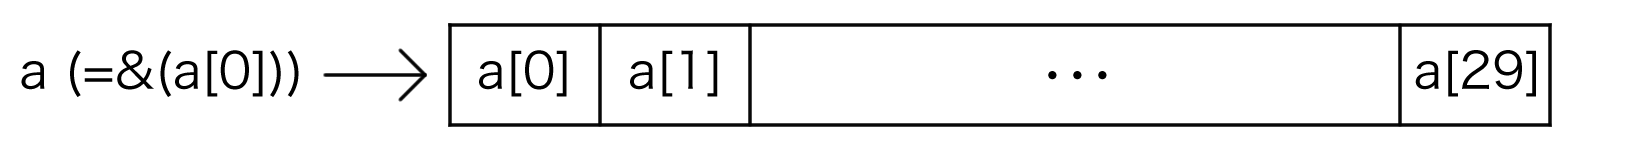
\includegraphics[width=10cm]{./a30.png}
\caption{int a{[}30{]}の図}
\end{figure}
int *a[30]は, int型を指すポインタ30個分の連続したメモリ240byteを確保する. 
aはその30個のポインタのメモリの先頭アドレスを表す. \\
図にすると以下のとおりである. 
\begin{figure}[H]
\centering
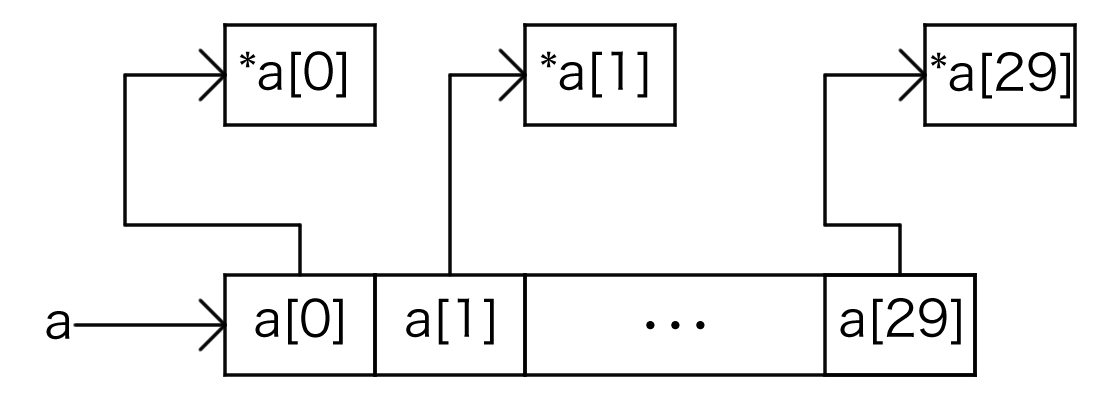
\includegraphics[width=7cm]{./pa30.png}
\caption{int *a{[}30{]}の図 \label{pa30}}
\end{figure}
\section*{課題10}
int **pのpはint型を指すポインタが格納されているアドレスである. 
図\ref{pa30}でいうとaのようなものである. \\
つまり以下のようになっている. \\
p $\rightarrow$ *p (int型を指すポインタ) $\rightarrow$ **p (int型変数)
%\nocite{*}
%\printbibliography[title=参考文献]
\end{document}


